\section{\sysname: Algorithm, Parallelism, and Work Partitioning}
\label{sec:algo}

We describe the \sysname algorithm, which includes several tweaks to \sysnameone
to reduce the number of non-matmul FLOPs.
We then describe how to parallelize the computation on different thread blocks
to make full use the GPU resources.
Finally we describe we partition the work between different warps within one
thread block to reduce the amount of shared memory access.
These improvements lead to 2-3$\times$ speedup as validated in~\cref{sec:experiments}.

\subsection{Algorithm}
\label{subsec:algo}

We tweak the algorithm from \sysnameone to reduce the number of non-matmul
FLOPs.
This is because modern GPUs have specialized compute units (e.g., Tensor Cores
on Nvidia GPUs) that makes matmul much faster.
As an example, the A100 GPU has a max theoretical throughput of 312 TFLOPs/s of
FP16/BF16 matmul, but only 19.5 TFLOPs/s of non-matmul FP32.
Another way to think about this is that each non-matmul FLOP is 16$\times$ more
expensive than a matmul FLOP.
To maintain high throughput (e.g., more than 50\% of the maximum theoretical
TFLOPs/s), we want to spend as much time on matmul FLOPs as possible.

\subsubsection{Forward pass}

We revisit the online softmax trick as shown in~\cref{subsec:flashv1} and make
two minor tweaks to reduce non-matmul FLOPs:
\begin{enumerate}
  \item We do not have to rescale both terms of the output update by $\diag(\ell^{(2)})^{-1}$:
  \begin{equation*}
    \vO^{(2)} = \diag(\ell^{(1)} / \ell^{(2)})^{-1} \vO^{(1)} + \diag(\ell^{(2)})^{-1} e^{\vS^{(2)} - m^{(2)}} \vV^{(2)}.
  \end{equation*}
  We can instead maintain an ``un-scaled'' version of $\vO^{(2)}$ and keep
  around the statistics $\ell^{(2)}$:
  \begin{equation*}
    \tilde{\vO}^{(2)} = \diag(\ell^{(1)})^{-1} \vO^{(1)} + e^{\vS^{(2)} - m^{(2)}} \vV^{(2)}.
  \end{equation*}
  Only at the every end of the loop do we scale the final
  $\tilde{\vO}^{(\mathrm{last})}$ by $\diag(\ell^{(\mathrm{last})})^{-1}$ to get
  the right output.

  \item We do not have to save both the max $m^{(j)}$ and the sum of
  exponentials $\ell^{(j)}$ for the backward pass. We only need to store the
  logsumexp $L^{(j)} = m^{(j)} + \log(\ell^{(j)})$.
\end{enumerate}

In the simple case of 2 blocks in~\cref{subsec:flashv1}, the online softmax
trick now becomes:
\begin{align*}
  m^{(1)} &= \mathrm{rowmax}(\vS^{(1)})  \in \mathbb{R}^{B_r}\\
  \ell^{(1)} &= \mathrm{rowsum}(e^{\vS^{(1)} - m^{(1)}}) \in \mathbb{R}^{B_r} \\
  \tilde{\vO^{(1)}} &= e^{\vS^{(1)} - m^{(1)}} \vV^{(1)} \in \mathbb{R}^{B_r \times d}\\
  m^{(2)} &= \max(m^{(1)}, \mathrm{rowmax}(\vS^{(2)})) = m \\
  \ell^{(2)} &= e^{m^{(1)} - m^{(2)}} \ell^{(1)} + \mathrm{rowsum}(e^{\vS^{(2)} - m^{(2)}}) = \mathrm{rowsum}(e^{\vS^{(1)} - m}) + \mathrm{rowsum}(e^{\vS^{(2)} - m}) = \ell \\
  \tilde{\vP}^{(2)} &= \diag(\ell^{(2)})^{-1} e^{\vS^{(2)} - m^{(2)}} \\
  \tilde{\vO}^{(2)} &= \diag(e^{m^{(1)} - m^{(2)}})^{-1} \tilde{\vO}^{(1)} + e^{\vS^{(2)} - m^{(2)}} \vV^{(2)} = e^{s^{(1)} - m} \vV^{(1)} + e^{s^{(2)} - m} \vV^{(2)} \\
  \vO^{(2)} &= \diag(\ell^{(2)})^{-1} \tilde{\vO}^{(2)} = \vO.
\end{align*}

We describe the full \sysname forward pass in~\cref{alg:flash2_fwd}.

\begin{algorithm}[H]
  % \algsetup{linenosize=\tiny}
  \caption{\small\label{alg:flash2_fwd}\sysname forward pass}
  \begin{algorithmic}[1]
    \REQUIRE Matrices $\vQ, \vK, \vV \in \mathbb{R}^{N \times d}$ in HBM, block sizes $B_c$, $B_r$.
    \STATE \label{alg:stream_attn_split_qkv} Divide $\vQ$ into $T_r = \left\lceil\frac{N}{B_r} \right\rceil$ blocks $\vQ_1, \dots, \vQ_{T_r}$ of size $B_r \times d$ each,
    and divide $\vK, \vV$ in to $T_c = \left\lceil \frac{N}{B_c} \right\rceil$ blocks $\vK_1, \dots, \vK_{T_c}$ and
    $\vV_1, \dots, \vV_{T_c}$, of size $B_c \times d$ each.
    \STATE Divide the output $\vO \in \mathbb{R}^{N \times d}$ into $T_r$ blocks $\vO_i, \dots, \vO_{T_r}$ of size
    $B_r \times d$ each, and divide the logsumexp $L$ into $T_r$ blocks $L_i, \dots, L_{T_r}$ of size
    $B_r$ each.
    \FOR{$1 \le i \le T_r$} \label{alg:stream_attn_outer_loop}
      \STATE \label{alg:stream_attn_load_q} Load $\vQ_i$ from HBM to on-chip SRAM.
      \STATE \label{alg:stream_attn_init} On chip, initialize $\vO_{i}^{(0)} = (0)_{B_r \times d} \in \mathbb{R}^{B_r \times d}, \ell_{i}^{(0)} = (0)_{B_r} \in \mathbb{R}^{B_r}, m_{i}^{(0)} = (-\infty)_{B_r} \in \mathbb{R}^{B_r}$.
      \FOR{$1 \le j \le T_c$}
        \STATE \label{alg:stream_attn_load_kv} Load $\vK_j, \vV_j$ from HBM to on-chip SRAM.
        \STATE \label{alg:stream_attn_qk} On chip, compute $\vS_{i}^{(j)} = \vQ_i \vK_j^T \in \mathbb{R}^{B_r \times B_c}$.
        \STATE \label{alg:stream_attn_statistics} On chip, compute
        $m_{i}^{(j)} = \mathrm{max}(m_{i}^{(j-1)}, \mathrm{rowmax}(\vS_{i}^{(j)})) \in \mathbb{R}^{B_r}$, $\tilde{\vP}_{i}^{(j)} = \exp(\vS_{i}^{(j)} - m_{i}^{(j)}) \in \mathbb{R}^{B_r \times B_c}$ (pointwise),
        $\ell_{i}^{(j)} = e^{m_{i}^{j-1} - m_{i}^{(j)}} \ell_{i}^{(j-1)} + \mathrm{row sum}(\tilde{\vP}_{i}^{(j)}) \in \mathbb{R}^{B_r}$.
        \STATE \label{alg:stream_attn_update} On chip, compute
        $\vO_{i}^{(j)} = \diag(e^{m_{i}^{(j-1)} - m_{i}^{(j)}})^{-1} \vO_{i}^{(j-1)} + \tilde{\vP}_{i}^{(j)} \vV_j$.
      \ENDFOR
      \STATE On chip, compute $\vO_{i} = \diag(\ell_{i}^{(T_c)})^{-1} \vO_{i}^{(T_c)}$.
      \STATE On chip, compute $L_{i} = m_{i}^{(T_c)} + \log(\ell_i^{(T_c)})$.
      \STATE Write $\vO_{i}$ to HBM as the $i$-th block of $\vO$.
      \STATE Write $L_{i}$ to HBM as the $i$-th block of $L$.
    \ENDFOR
    \STATE Return the output $\vO$ and the logsumexp $L$.
  \end{algorithmic}
\end{algorithm}

\paragraph{Causal masking.}

One common use case of attention is in auto-regressive language modeling, where
we need to apply a causal mask to the attention matrix $\vS$ (i.e., any entry
$\vS_{ij}$ with $j > i$ is set to $-\infty$).
\begin{enumerate}
  \item As \sysnameone and \sysname already operate by blocks, for any blocks
  where all the column indices are more than the row indices (approximately half
  of the blocks for large sequence length), we can skip the computation of that
  block.
  This leads to around 1.7-1.8$\times$ speedup compared to attention without the
  causal mask.
  \item We do not need to apply the causal mask for blocks whose row indices are
  guaranteed to be strictly less than the column indices. This means that for
  each row, we only need apply causal mask to 1 block (assuming square block).
\end{enumerate}

\paragraph{Correctness, runtime, and memory requirement.}
As with \sysnameone, \cref{alg:flash2_fwd} returns the correct output
$\vO = \softmax(\vQ\vK^\top)\vV$ (with no approximation), using $O(N^2d)$ FLOPs and
requires $O(N)$ additional memory beyond inputs and output (to store the
logsumexp $L$).
The proof is almost the same as the proof of
\citet[Theorem 1]{dao2022flashattention}, so we omit it here.

\subsubsection{Backward pass}

The backward pass of \sysname is almost the same as that of \sysnameone. We make
a minor tweak to only use the row-wise logsumexp $L$ instead of both the
row-wise max and row-wise sum of exponentials in the softmax.
We include the backward pass description in~\cref{alg:flash_bwd} for completeness.
\begin{algorithm}[h]
  \caption{\small\label{alg:flash_bwd}\sysname Backward Pass}
  \begin{algorithmic}[1]
    \REQUIRE Matrices $\vQ, \vK, \vV, \vO, \vdO \in \mathbb{R}^{N \times d}$ in HBM,
    vector $L \in \mathbb{R}^N$ in HBM, block sizes $B_c$, $B_r$.
    \STATE Divide $\vQ$ into $T_r = \left\lceil\frac{N}{B_r} \right\rceil$ blocks $\vQ_1, \dots, \vQ_{T_r}$ of size $B_r \times d$ each,
    and divide $\vK, \vV$ in to $T_c = \left\lceil \frac{N}{B_c} \right\rceil$ blocks $\vK_1, \dots, \vK_{T_c}$ and
    $\vV_1, \dots, \vV_{T_c}$, of size $B_c \times d$ each.
    \STATE Divide $\vO$ into $T_r$ blocks $\vO_i, \dots, \vO_{T_r}$ of size
    $B_r \times d$ each, divide $\vdO$ into $T_r$ blocks $\vdO_i, \dots, \vdO_{T_r}$
    of size $B_r \times d$ each, and divide $L$ into $T_r$ blocks $L_i, \dots, L_{T_r}$ of size
    $B_r$ each.
    \STATE Initialize $\vdQ = (0)_{N \times d}$ in HBM and divide it into $T_r$ blocks $\vdQ_1, \dots, \vdQ_{T_r}$ of size $B_r \times d$ each.
    Divide $\vdK, \vdV \in \mathbb{R}^{N \times d}$ in to $T_c$ blocks $\vdK_1, \dots, \vdK_{T_c}$ and
    $\vdV_1, \dots, \vdV_{T_c}$, of size $B_c \times d$ each.
    \STATE Compute $D = \mathrm{rowsum}(\vdO \circ \vO) \in \mathbb{R}^d$ (pointwise multiply), write
    $D$ to HBM and divide it into $T_r$ blocks $D_1, \dots, D_{T_r}$ of size
    $B_r$ each.
    \FOR{$1 \le j \le T_c$}
      \STATE Load $\vK_j, \vV_j$ from HBM to on-chip SRAM.
      \STATE Initialize $\vdK_j = (0)_{B_c \times d}, \vdV_j = (0)_{B_c \times d}$ on SRAM.
      \FOR{$1 \le i \le T_r$}
        \STATE Load $\vQ_i, \vO_i, \vdO_i, \vdQ_i, L_i, D_i$ from HBM to on-chip SRAM.
        \STATE On chip, compute $\vS_{i}^{(j)} = \vQ_i \vK_j^T \in \mathbb{R}^{B_r \times B_c}$.
        \STATE On chip, compute $\vP_{i}^{(j)} = \exp(\vS_{ij} - L_{i}) \in \mathbb{R}^{B_r \times B_c}$.
        \STATE On chip, compute
        $\vdV_j \leftarrow \vdV_j + (\vP_{i}^{(j)})^\top \vdO_i \in \mathbb{R}^{B_c \times d}$.
        \STATE On chip, compute
        $\vdP_{i}^{(j)} = \vdO_{i} \vV_j^\top \in \mathbb{R}^{B_r \times B_c}$.
        \STATE On chip, compute $\vdS_{i}^{(j)} = \vP_{i}^{(j)} \circ (\vdP_{i}^{(j)} - D_i) \in \mathbb{R}^{B_r \times B_c}$.
        \STATE Load $\vdQ_i$ from HBM to SRAM, then on chip, update
        $\vdQ_{i} \leftarrow \vdQ_i + \vdS_{i}^{(j)} \vK_j \in \mathbb{R}^{B_r \times d}$, and write
        back to HBM.
        \STATE On chip, compute $\vdK_{j} \leftarrow \vdK_j + {\vdS_{i}^{(j)}}^\top \vQ_i \in \mathbb{R}^{B_c \times d}$.
      \ENDFOR
      \STATE Write $\vdK_j, \vdV_j$ to HBM.
    \ENDFOR
    \STATE Return $\vdQ, \vdK, \vdV$.
  \end{algorithmic}
\end{algorithm}

\paragraph{Multi-query attention and grouped-query attention.}
Multi-query attention (MQA)~\citep{shazeer2019fast} and grouped-query attention
(GQA)~\citep{ainslie2023gqa} are variants of attention where multiple heads of
query attend to the same head of key and value, in order to reduce the size of
KV cache during inference.
Instead of having to duplicate the key and value heads for the computation, we
implicitly manipulate the indices into the head to perform the same computation.
In the backward pass, we need to sum the gradients $\vdK$ and $\vdV$ across
different heads that were implicitly duplicated.

\subsection{Parallelism}
\label{subsec:parallelism}

The first version of \sysnameone parallelizes over batch size and number of
heads.
We use 1 thread block to process one attention head, and there are overall
$\text{batch size} \cdot \text{number of heads}$ thread blocks.
Each thread block is scheduled to run on a streaming multiprocessor (SM), and
there are 108 of these SMs on an A100 GPU for example.
This scheduling is efficient when this number is large (say $\geq 80$), since we
can effectively use almost all of the compute resources on the GPU.

In the case of long sequences (which usually means small batch sizes or small
number of heads), to make better use of the multiprocessors on the GPU, we now
additionally parallelize over the sequence length dimension.
This results in significant speedup for this regime.


\paragraph{Forward pass.}
We see that the outer loop (over sequence length) is embarrassingly parallel,
and we schedule them on different thread blocks that do not need to communicate
with each other.
We also parallelize over the batch dimension and number of heads dimension, as
done in \sysnameone.
The increased parallelism over sequence length helps improve occupancy (fraction
of GPU resources being used) when the batch size and number of heads are small,
leading to speedup in this case.

These ideas of swapping the order of the loop (outer loop over row blocks and
inner loop over column blocks, instead of the other way round in the original
\sysnameone paper), as well as parallelizing over the sequence length dimension
were first suggested and implemented by Phil Tillet in the
Triton~\citep{tillet2019triton}
implementation.\footnote{\url{https://github.com/openai/triton/blob/main/python/tutorials/06-fused-attention.py}}

\paragraph{Backward pass.}
Notice that the only shared computation between different column blocks is in
update $\vdQ$ in \cref{alg:flash_bwd}, where we need to load $\vdQ_i$ from HBM
to SRAM, then on chip, update
$\vdQ_{i} \leftarrow \vdQ_i + \vdS_{i}^{(j)} \vK_j$, and write back to HBM.
We thus parallelize over the sequence length dimension as well, and schedule 1
thread block for each column block of the backward pass.
We use atomic adds to communicate between different thread blocks to update $\vdQ$.

We describe the parallelization scheme in \cref{fig:parallelism}.
\begin{figure}[ht]
  \centering
  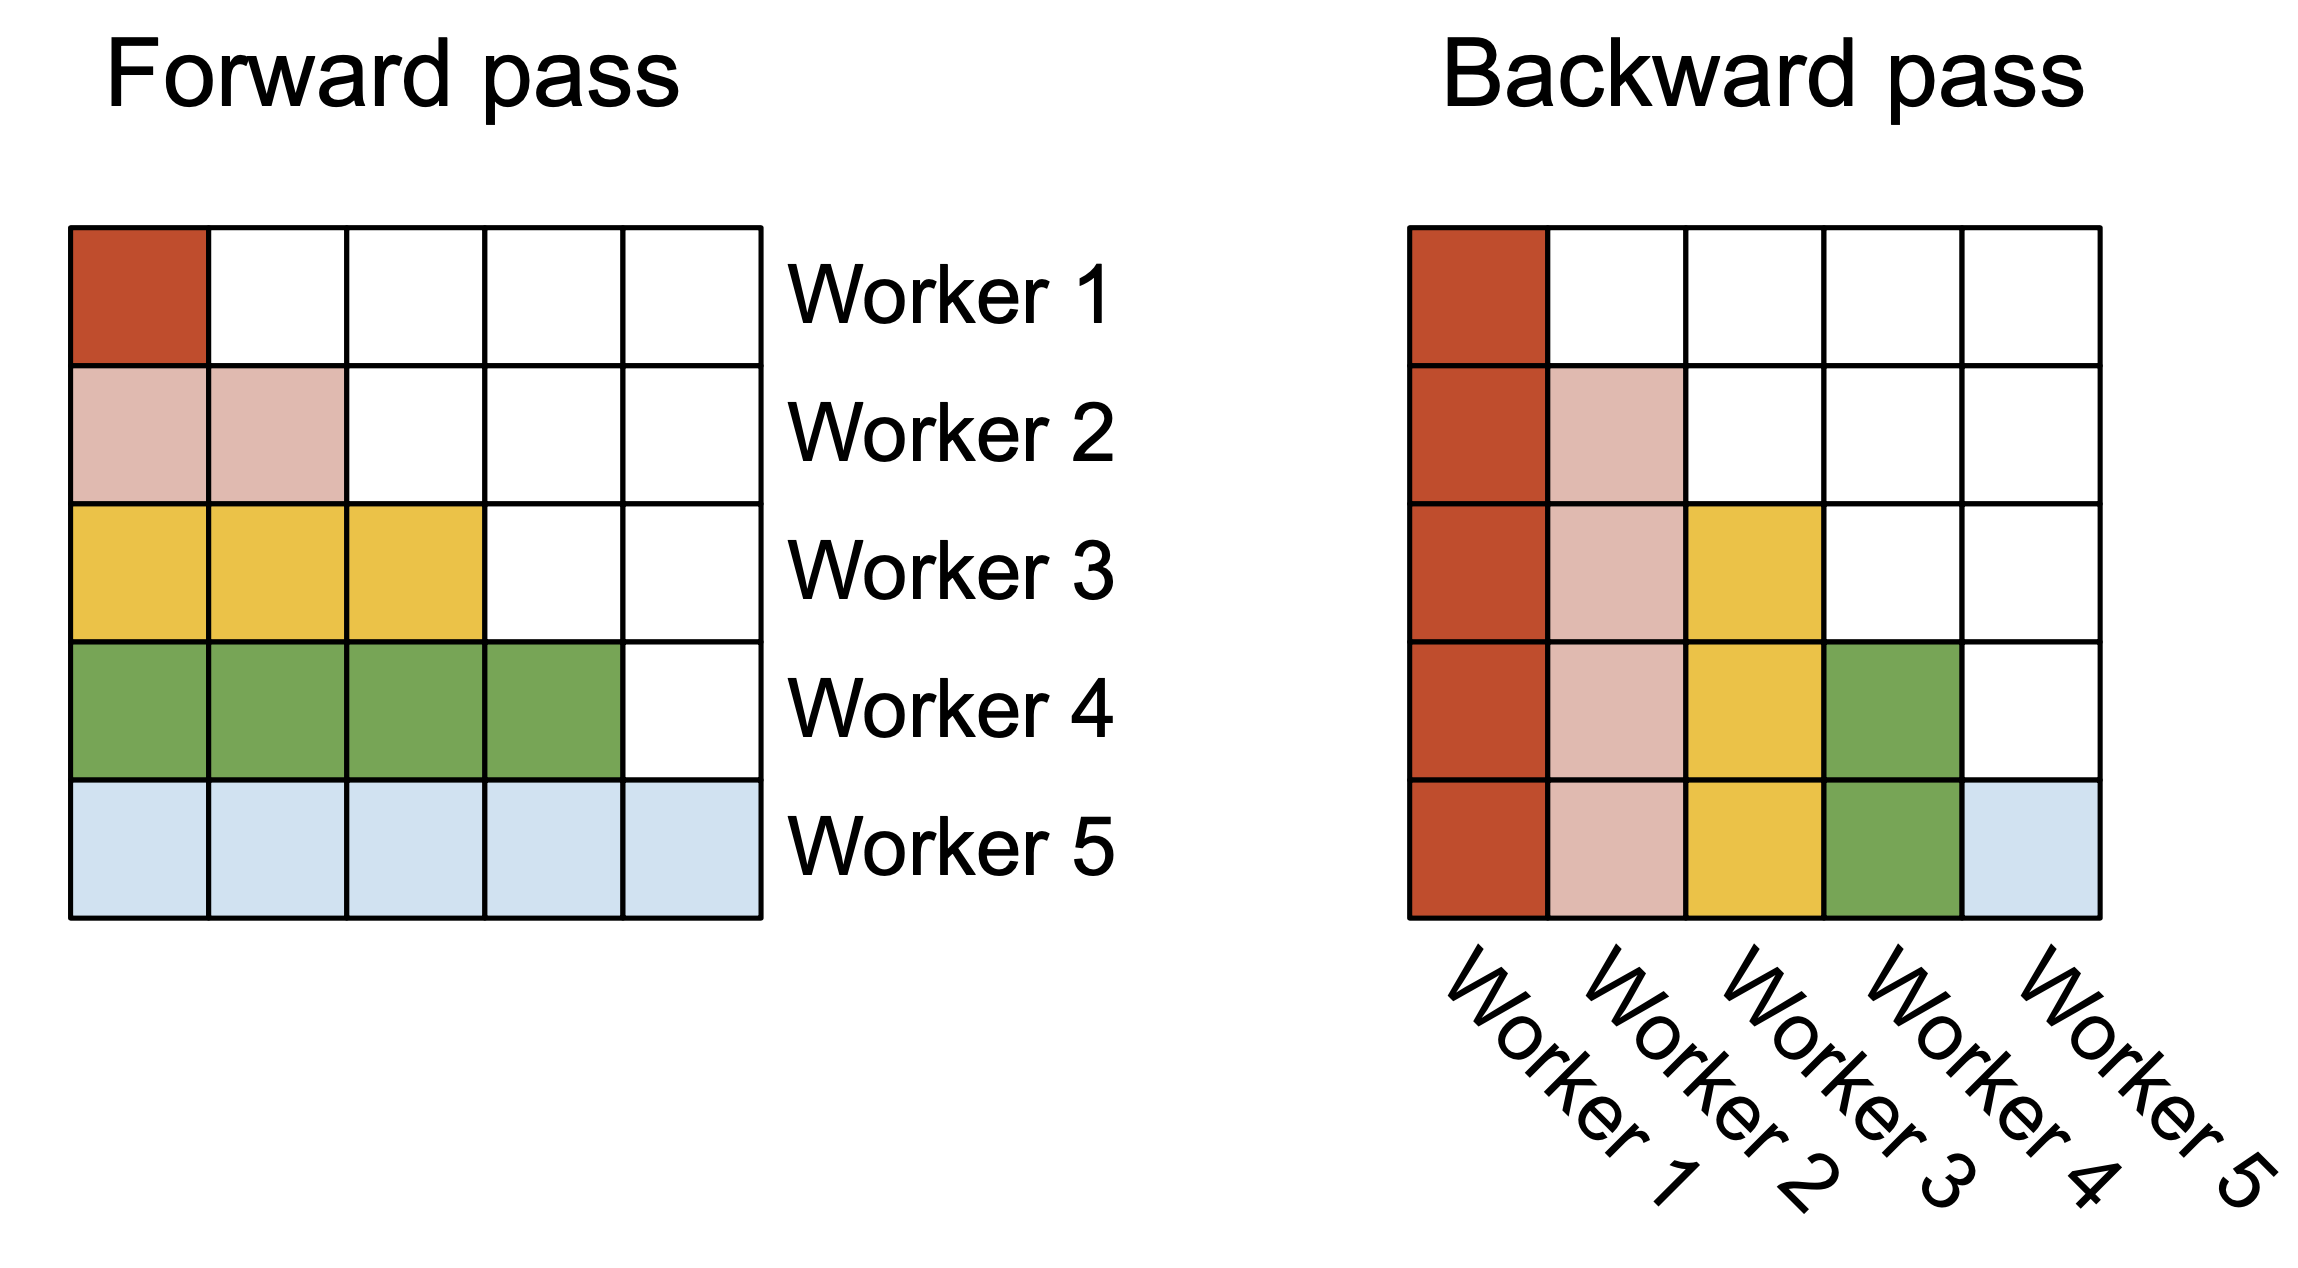
\includegraphics[width=0.95\linewidth]{figs/flashattention_fwd_bwd_parallel.png}
  \caption{\label{fig:parallelism}In the forward pass (left), we parallelize the
    workers (thread blocks) where each worker takes care of a block of rows of
    the attention matrix.
    In the backward pass (right), each worker takes care of a block of columns
    of the attention matrix.}
\end{figure}


\subsection{Work Partitioning Between Warps}
\label{subsec:work_partitioning}

As \cref{subsec:parallelism} describe how we schedule thread blocks, even within
each thread block, we also have to decide how to partition the work between
different warps.
We typically use 4 or 8 warps per thread block, and the partitioning is described
in \cref{fig:partitioning}.

\paragraph{Forward pass.}
For each block, \sysnameone splits $\vK$ and $\vV$ across 4 warps while keeping
$\vQ$ accessible by all warps.
Each warp multiplies to get a slice of $\vQ \vK^\top$, then they need to multiply
with a slice of $\vV$ and communicate to add up the result.
This is referred to as the ``split-K'' scheme.
However, this is inefficient since all warps need to write their intermediate
results out to shared memory, synchronize, then add up the intermediate results.
These shared memory reads/writes slow down the forward pass in \sysnameone.

In \sysname, we instead split $\vQ$ across 4 warps while keeping $\vK$ and $\vV$
accessible by all warps.
After each warp performs matrix multiply to get a slice of $\vQ \vK^\top$, they just need to
multiply with their shared slice of $\vV$ to get their corresponding
slice of the output.
There is no need for communication between warps.
The reduction in shared memory reads/writes yields speedup (\cref{sec:experiments}).

\begin{figure}[ht]
  \centering
  \begin{subfigure}{.53\textwidth}
    \centering
    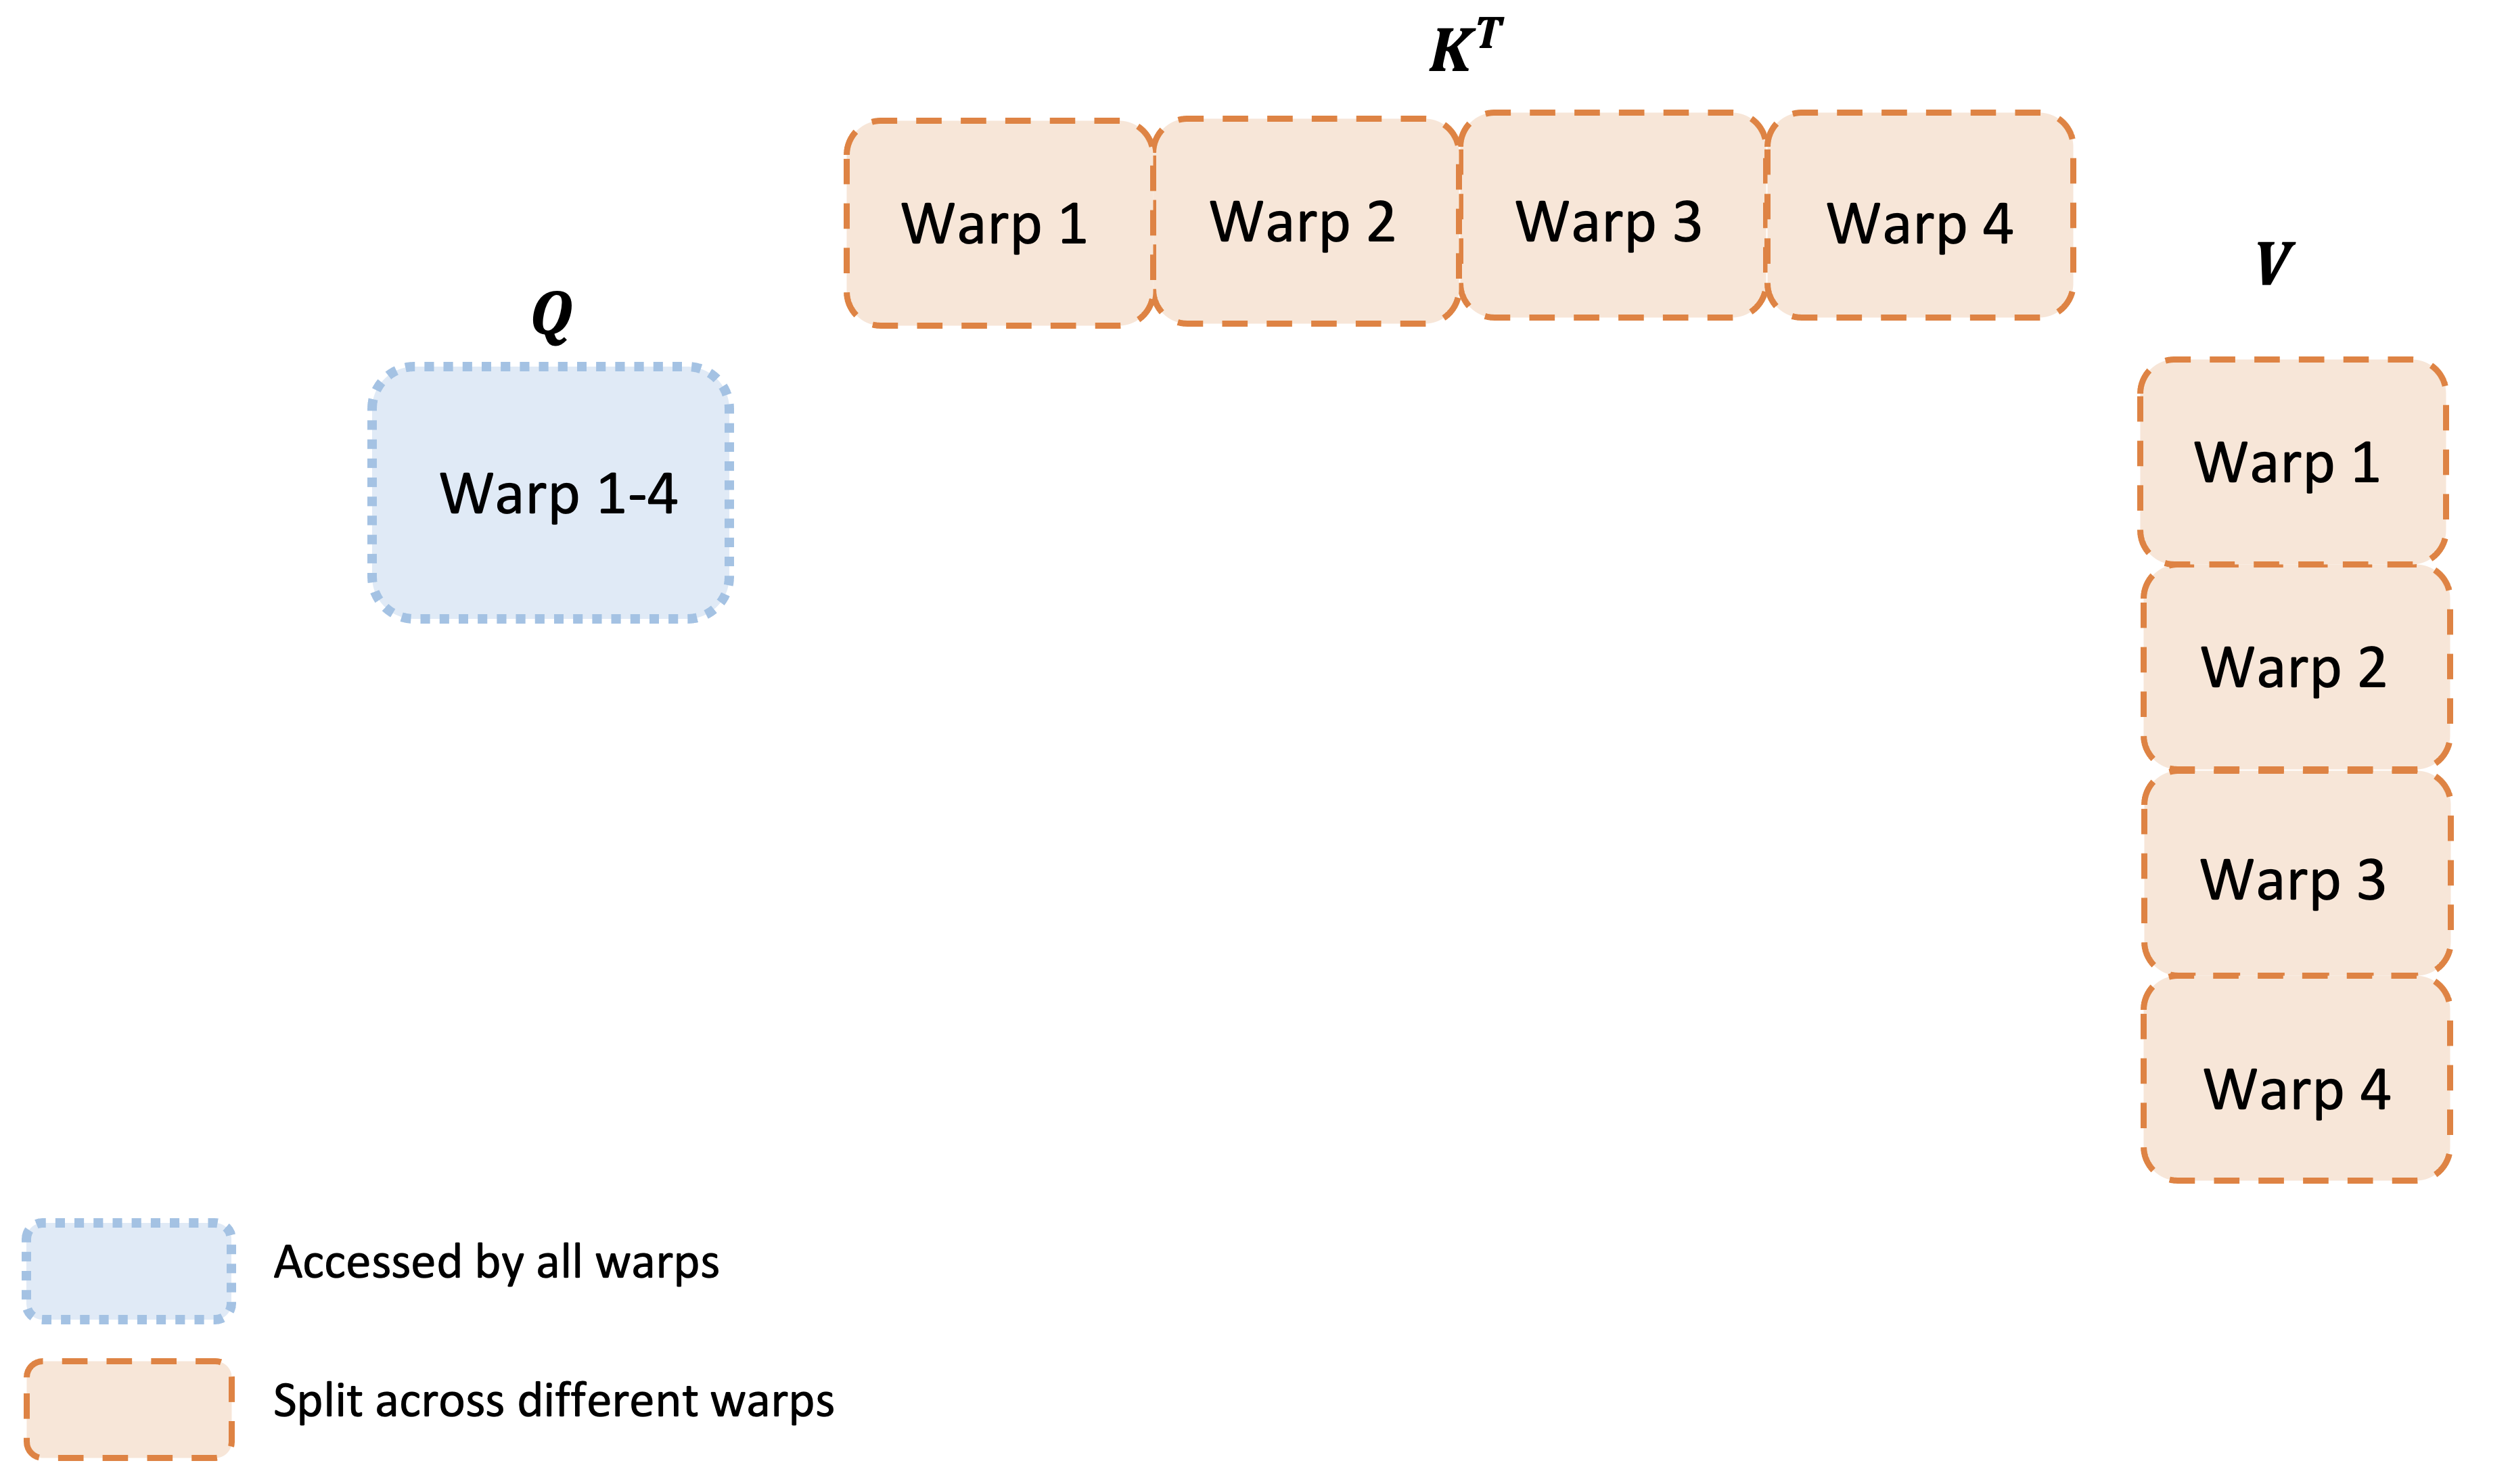
\includegraphics[width=.95\linewidth]{figs/flash_partitioning.png}
    \caption{\sysnameone}
  \end{subfigure}%
  \begin{subfigure}{.47\textwidth}
    \centering
    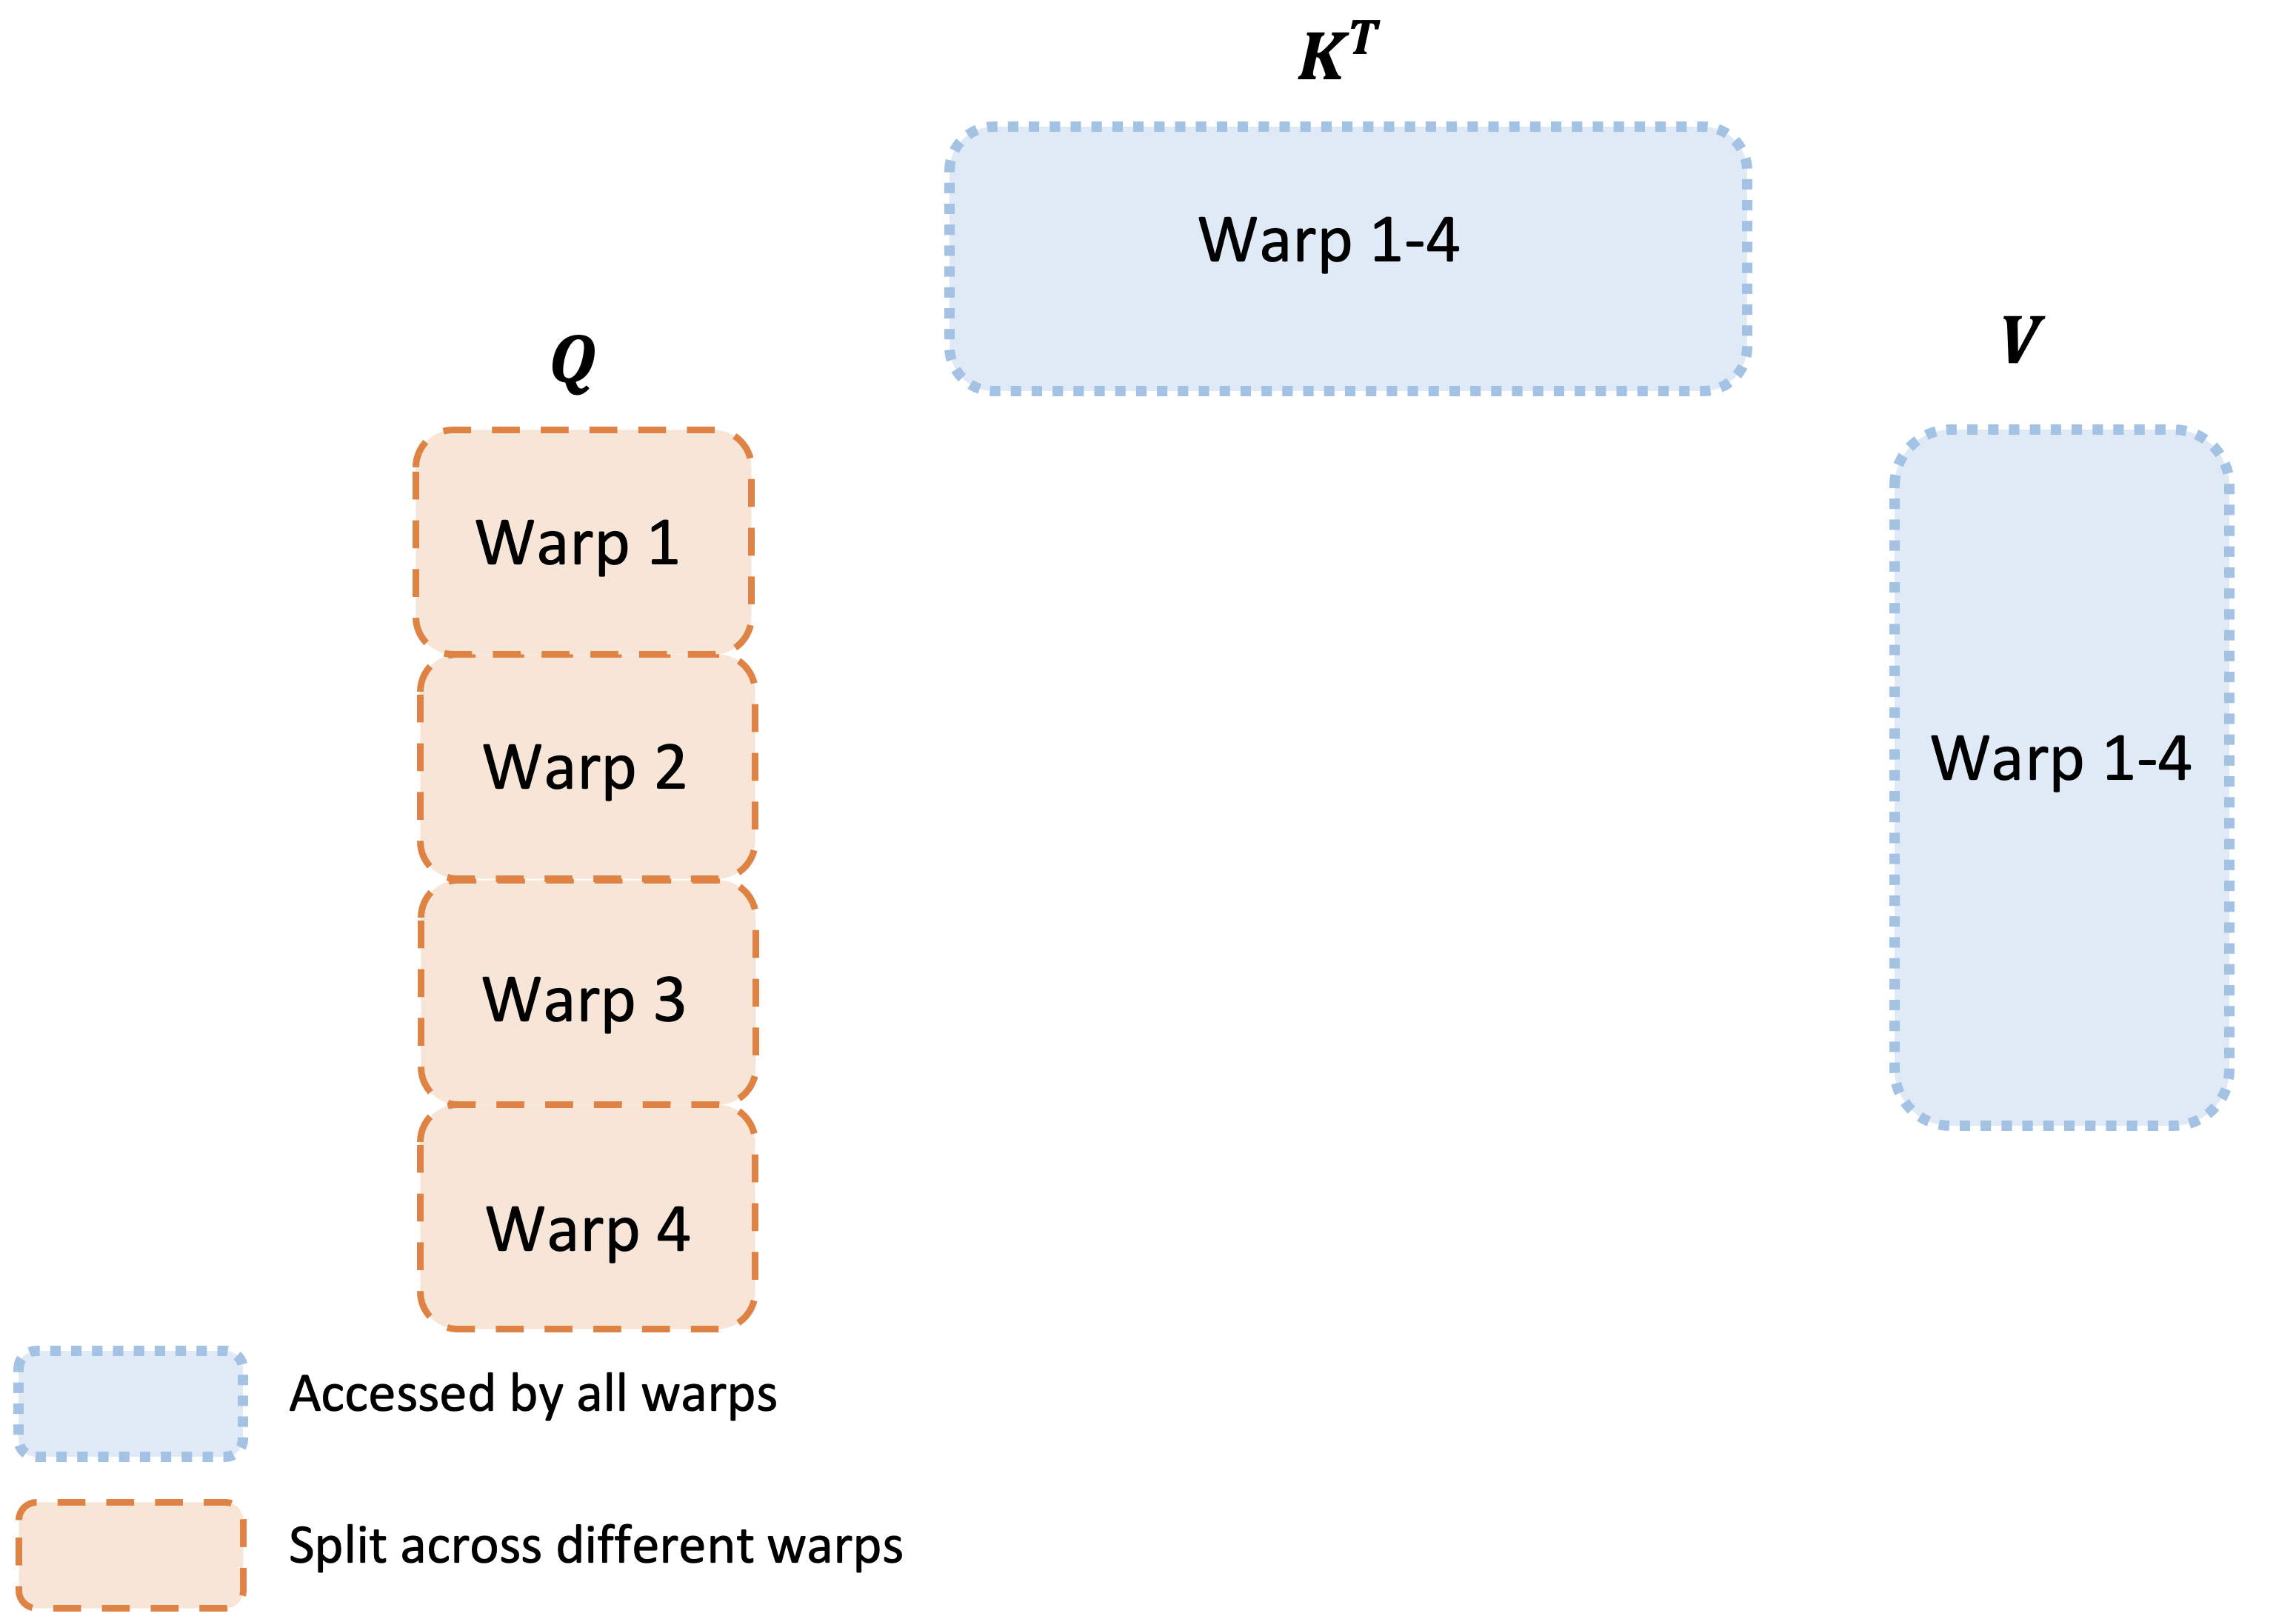
\includegraphics[width=.95\linewidth]{figs/flash2_partitioning.png}
    \caption{\sysname}
  \end{subfigure}
  \caption{Work partitioning between different warps in the forward pass}
  \label{fig:partitioning}
\end{figure}

\paragraph{Backward pass.}
Similarly for the backward pass, we choose to partition the warps to avoid the
``split-K'' scheme.
However, it still requires some synchronization due to the more complicated
dependency between all the different inputs and gradients
$\vQ, \vK, \vV, \vO, \vdO, \vdQ, \vdK, \vdV$.
Nevertheless, avoiding ``split-K'' reduces shared memory reads/writes and again
yields speedup (\cref{sec:experiments}).

\paragraph{Tuning block sizes}
Increasing block sizes generally reduces shared memory loads/stores, but
increases the number of registers required and the total amount of shared
memory.
Past a certain block size, register spilling causes significant slowdown, or the
amount of shared memory required is larger than what the GPU has available, and
the kernel cannot run at all.
Typically we choose blocks of size $\{64, 128\} \times \{64, 128\}$, depending on the
head dimension $d$ and the device shared memory size.

We manually tune for each head dimensions since there are essentially only 4
choices for block sizes, but this could benefit from auto-tuning to avoid this
manual labor.
We leave this to future work.